% homework/hw10x/hw10x.tex
% Year 7 - Extra Homework 10 (Science Models). Why Is Mr Bowen Still Awake?
%
% Goes out alongside Homework 10. It began as a stand-alone "challenge" in
% homework/caffeine and was renamed Extra Homework 10 on 24 Oct 2026.
%
% EIGHT PAGES (two A4 sheets, double-sided). Goes home after Coffee, Carbon
% and Stars (content/y7-science/U03_coffee). Every number is the deck's:
% caffeine's half-life about 5 hours, a cup of coffee about 100 mg, carbon-14's
% half-life 5 700 years, carbon dating up to about 50 000 years, dinosaurs 66
% million years ago, the Sun about 4.6 billion years old with about half its
% core hydrogen gone (71% at birth, 34% now).
%
% REWRITTEN 24 Oct 2026, EASIER. The teacher found the first version too hard
% for Year 7. The deck only ever HALVES (its plan: "keep the maths to
% halving"), so this sheet now does too. Out: the hour-by-hour rule (x 0.87
% every hour) and everything built on it -- the 20-row table, the graph with a
% scale to choose -- the latte added halfway through Mr Bowen's day, the
% 400 mg daily limit, the label-maths drill, and the charcoal and cotton traps
% in the museum. Kept, by request: the interview, and students still look the
% caffeine up themselves, on the label or with Google. In, by request: the Sun
% and "different speeds, the same maths" (deck slides 20-22).
%
%   Part A  Mr Bowen's coffee. Two cold brews at 8 a.m. (400 mg), bed at
%           11 p.m.: 400, 200, 100, 50, every 5 hours. The graph is plotted
%           from those four dots, and 8 p.m. is read between them (deck slide
%           5). Does it ever run out? The limitation, as a fill-in (slide 6).
%   Part B  Interview one adult about ONE drink (their first caffeine drink
%           yesterday), look it up, halve it every 5 hours past bedtime, and
%           estimate their bedtime caffeine between two boxes. A worked tea
%           example (40 mg at 7 a.m.) shows the clock crossing noon and
%           midnight.
%   Part C  Carbon dating: the chain in years, a five-row museum (a stone axe
%           was never alive; a T. rex tooth is too old), two fill-ins.
%   Part D  The Sun: half of 71% against 34%, hydrogen into helium, three
%           clocks to match and put in order.
%   Part E  Caffeine and sleep, on its own last page (added 24 Oct at the
%           teacher's request, replacing a same/different question whose
%           starter gave the answer, a joke tick question and a checklist):
%           a six-point reading guide (adenosine, named; 100 mg near bedtime
%           for an adult, about 50 mg for a child; stop 8 hours before bed),
%           a plan from the packet's numbers (50 mg at 11 p.m., one cup by
%           3 p.m., one cold brew leaves 25 mg), and a letter to Mr Bowen with
%           six tick-off conditions and NO sentence starter (teacher's call).
%
% FRENCH COPY (26 Oct 2026). hw10x-fr.pdf is this file built with \FRENCH
% defined: HW 9's scheme (see hw09/README.md). \fr{...} prints a grey French
% line under the English, \frin{...} a short French gloss in brackets, and
% \frnode{...} a French line under a drawing's label. All three are EMPTY in
% the English copy, so the English layout is the one checked to eight pages.
% The English key word stays inside the French line, in blue; numbers keep the
% English decimal point; times are said the French way that matches the
% sheet's 12-hour clock (11 p.m. = 11 h du soir). An English "billion" is a
% French "milliard", and Part D's word help says so. The key stays English.
%
% House style is shared: see homework/hw-style.tex. Method: the new-homework
% skill. Source is pure ASCII on purpose: French accents are written \'e etc.
%
% Build:  pwsh .claude/skills/new-homework/scripts/build-hw.ps1 hw10x -French

\documentclass[12pt,a4paper]{article}

% -- Answer key switch -------------------------------------------------------
\newif\ifkey
\ifdefined\TEACHER\keytrue\else
  \keyfalse        % \keyfalse = student copy   |   \keytrue = teacher copy
\fi

% -- Language switch ---------------------------------------------------------
% The French copy (hw10x-fr.pdf) is this file built with \FRENCH defined. See
% hw09/README.md for the scheme.
\newif\iffr
\ifdefined\FRENCH\frtrue\fi

% -- House style -------------------------------------------------------------
% homework/hw-style.tex
% Shared house style for every Year 7 homework packet. \input this from the
% packet file, right after \documentclass and the answer-key switch.
%
% Do not fork this file per packet. If a packet needs a different look, the
% question is whether every packet should have it.
%
% The choices here are deliberate and were arrived at by printing and looking:
%   * No solid dark banners. Every header is a light tint with a coloured spine
%     on the left, so colour reads clearly without flooding a school printer.
%   * No marks and no mark totals. These are practice, not exam papers.
%   * Lato at 12pt with open leading, plus mathastext so inline maths is Lato
%     too. Without mathastext every "-6 + 4" is Computer Modern serif and the
%     sheet looks half-typeset.
%   * Writing lines are spaced for Year 7 handwriting, not adult margin notes.
%   * Pages fill. \needspace is redefined below so a heading no longer drags
%     the page break up to itself, and every heading is glued to the box under
%     it. Packets built before 2026-09-30 were laid out under the old rules and
%     will reflow if rebuilt -- re-read every page if you rebuild one.
%
% Provides: \wlines \blank \tickbox \sep \qmk-free marks (none) \hwsection
% \qhead \expr, the workspace box, and the remember / wordhelp / activity /
% yourturn coloured boxes. Palette matches the lesson decks exactly.

% -- Packages ----------------------------------------------------------------
\usepackage[T1]{fontenc}
\usepackage[utf8]{inputenc}
\usepackage[default]{lato}
\usepackage[a4paper,top=1.7cm,bottom=1.7cm,left=2.0cm,right=2.0cm,headheight=15pt]{geometry}
\usepackage{amsmath,amssymb}
\usepackage{xcolor}
\usepackage[most]{tcolorbox}
\usepackage{enumitem}
\usepackage{tikz}
\usetikzlibrary{arrows.meta}
\usepackage{array}
\usepackage{tabularx}
\usepackage{fancyhdr}
\usepackage{multicol}
\usepackage{needspace}
\usepackage{graphicx}

% Make maths use Lato too. Without this, every "-6 + 4" on the page is set in
% Computer Modern serif and the sheet looks half-typeset. Must come last.
\usepackage[italic]{mathastext}

% -- \needspace, without the hole it used to leave ----------------------------
% needspace.sty writes "\vskip 0pt plus X \penalty-100" in front of every
% heading. A page that ends anywhere else is underfull with no stretch, so TeX
% scores it b=10000; a page that ends AT a heading gets that X of stretch and a
% finite badness, and wins. So any heading in roughly the bottom half of a page
% claimed the break, and the question under it moved over whole, leaving a hole
% the size of the question. \tracingpages showed it exactly (b=4531 at the
% heading, b=10000 at every later break) while building homework/q1rev, and it
% is where the half-empty pages in HW 1-8 came from.
% This keeps only the \penalty9999, which still refuses to put a heading in the
% last X of a page. Keeping a heading WITH the box under it is \nobreak's job
% now -- see \hwsection and \qhead below.
\makeatletter
\renewcommand{\needspace}[1]{\begingroup\setlength{\dimen@}{#1}%
  \vskip\dimen@\penalty9999\vskip-\dimen@\endgroup}
\makeatother

\linespread{1.06}\selectfont

% -- The Learner's Book palette (same hex values as the lesson decks) ---------
\definecolor{cbteal}{HTML}{0087A8}
\definecolor{cbpurple}{HTML}{5C2483}
\definecolor{cborange}{HTML}{C25E12}
\definecolor{cbgreen}{HTML}{4A8B23}
\definecolor{cbred}{HTML}{C8102E}
\definecolor{cbblue}{HTML}{1A5FA8}
\definecolor{rulegray}{HTML}{9AA5AD}

% -- Answer lines and blanks -------------------------------------------------
% \wlines{n} draws n ruled writing lines, spaced wide enough for Year 7
% handwriting rather than for an adult with a fine pen.
\makeatletter
\newcommand{\wlines}[1]{%
  \par\vspace{0.75em}%
  \@tempcnta=0\relax
  \@whilenum\@tempcnta<#1\do{%
    \hbox to \linewidth{\color{rulegray}\leaders\hrule height 0.5pt\hfill}%
    \vspace{1.5em}%
    \advance\@tempcnta by 1\relax}%
  \par\vspace{-0.8em}%
}
\makeatother

% \blank[width] is an inline gap to write a short answer in.
\newcommand{\blank}[1][2.6cm]{\underline{\hspace{#1}}}

% A boxed space for showing working.
\newtcolorbox{workspace}[1][3.4cm]{%
  colback=white, colframe=rulegray, boxrule=0.5pt, arc=5pt,
  height=#1, left=6pt, right=6pt, top=4pt, bottom=4pt,
  before skip=9pt, after skip=11pt}

% An empty tick box.
\newcommand{\tickbox}{\fbox{\rule{0pt}{1.15em}\rule{1.15em}{0pt}}}

% A middot separator.
\newcommand{\sep}{\,\textperiodcentered\,}

% -- Section and question headings -------------------------------------------
% Light tint plus a fat coloured spine on the left. No solid dark banner: the
% colour reads clearly but barely costs the printer anything.
% needspace keeps a heading out of the last few lines of a page. The \nobreak
% after it keeps it with whatever comes next: a remember or word-help box that
% does not fit takes its heading over with it, instead of leaving the heading
% alone at the foot of the page. (The old needspace did that by accident, and
% left a hole every time; see above.)
\newcommand{\hwsection}[2][cbteal]{%
  \needspace{8\baselineskip}%
  \par\vspace{13pt}%
  \noindent
  \begin{tcolorbox}[enhanced, nobeforeafter, width=\textwidth,
      colback=#1!7, colframe=#1!7, arc=5pt,
      borderline west={5pt}{0pt}{#1},
      left=14pt, right=10pt, top=7pt, bottom=7pt]
    {\large\bfseries\color{#1}#2}
  \end{tcolorbox}%
  \par\nobreak\vspace{9pt}}

% \qhead[colour]{A2}{Moving along the line} -- a question heading.
\newcommand{\qhead}[3][cbteal]{%
  \needspace{6\baselineskip}%
  \par\vspace{11pt}%
  \noindent{\large\bfseries\color{#1}#2}\quad{\large\bfseries #3}\par\nobreak\vspace{4pt}}

% -- Coloured boxes ----------------------------------------------------------
% Shared look: rounded, light fill, coloured rule, coloured title text on a
% pale title strip rather than a dark one.
% NOT breakable. A breakable box that cannot fit its first lines forces its own
% page break, and \nobreak cannot stop a forced break -- so the heading above
% it was left alone at the foot of the page (tested: it happens with \nobreak
% in place). Unbreakable, the page builder moves heading and box together.
% These boxes are a few lines each; none needs to split.
\tcbset{hwbox/.style={
  enhanced, arc=6pt, boxrule=1pt,
  left=11pt, right=11pt, top=8pt, bottom=8pt,
  fonttitle=\bfseries, attach boxed title to top left={xshift=12pt, yshift=-8pt},
  boxed title style={arc=4pt, boxrule=1pt, left=7pt, right=7pt, top=2pt, bottom=2pt},
  top=13pt}}

% Orange: things to remember. Matches the deck's "Write This Down".
\newtcolorbox{remember}[1][Remember from the lesson]{hwbox,
  colback=cborange!6, colframe=cborange, coltitle=cborange,
  colbacktitle=white, title={#1}}

% Blue: English help. The barrier in this class is the wording, not the maths.
\newtcolorbox{wordhelp}[1][Word help]{hwbox,
  colback=cbblue!6, colframe=cbblue, coltitle=cbblue,
  colbacktitle=white, title={#1}}

% Purple: an activity or instruction.
\newtcolorbox{activity}[1][How to do this homework]{hwbox,
  colback=cbpurple!6, colframe=cbpurple, coltitle=cbpurple,
  colbacktitle=white, title={#1}}

% Green: your turn / a friendly nudge.
\newtcolorbox{yourturn}[1][Your turn]{hwbox,
  colback=cbgreen!7, colframe=cbgreen, coltitle=cbgreen!75!black,
  colbacktitle=white, title={#1}}

% -- Shorthands --------------------------------------------------------------
\newcommand{\dC}{\,^{\circ}\mathrm{C}}          % use inside maths: $-8\dC$
\newcommand{\key}[1]{{\color{cborange}\textbf{#1}}}
\newcommand{\eng}[1]{{\color{cbblue}\textbf{#1}}}

\setlist[enumerate]{itemsep=8pt, topsep=5pt, leftmargin=*}
\setlist[itemize]{itemsep=4pt, topsep=4pt, leftmargin=*}
\renewcommand{\arraystretch}{1.45}

% -- An expression the student is asked to work from -------------------------
\newcommand{\expr}[1]{%
  \tcbox[on line, colback=cbgreen!10, colframe=cbgreen!55, boxrule=1pt, arc=4pt,
         left=9pt, right=9pt, top=4pt, bottom=4pt]{\large\bfseries $#1$}}

% -- Running head and foot ---------------------------------------------------
% The packet overrides \fancyhead[L] with its own title.
\pagestyle{fancy}
\fancyhf{}
\fancyhead[L]{\small\color{black!55}Year 7\sep Homework}
\fancyhead[R]{\small\color{black!55}Name: \blank[3.4cm]}
\fancyfoot[C]{\small\color{black!55}Page \thepage}
\renewcommand{\headrulewidth}{0pt}
\renewcommand{\headrule}{\vspace{2pt}\hbox to\headwidth{\color{cbteal!45}\leaders\hrule height 1.2pt\hfill}}


\usepackage{colortbl}   % \rowcolor for the table headers

% -- French support lines ----------------------------------------------------
% \fr{...}  a French line of its own, grey and italic, under the English.
% \frin{...} a French gloss in brackets, inline -- for table cells and labels.
% \fq{...}  French quotation marks.
% Both start with \unskip: the line break before \fr is a space, and in the
% English copy it would otherwise sit at the end of the line and move a break.
% \fr has a \nobreak, so a French line never starts the page after its English
% (B1's third question did).
\newcommand{\fr}[1]{\unskip\iffr\par\nobreak\vspace{1pt}\noindent{\small\itshape\color{black!60}#1}\par\fi}
\newcommand{\frin}[1]{\unskip\iffr\ {\small\itshape\color{black!60}(#1)}\fi}
\newcommand{\fq}[1]{\guillemotleft\,#1\,\guillemotright}
% \frcell{...} a French line of its own inside a table cell (C2's objects).
\newcommand{\frcell}[1]{\unskip\iffr\par{\small\itshape\color{black!60}#1}\fi}
% \frnode{...} one more line under a TikZ label, French copy only. The node
% must have align= set. One line per call, so no \\ sits inside a group.
\newcommand{\frnode}[1]{\iffr\\[1pt]{\footnotesize\itshape\color{black!60}#1}\fi}
% \frl{english}{french}: a number of writing lines that is bigger in the
% French copy.
\newcommand{\frl}[2]{\iffr#2\else#1\fi}

% "8 a.m. Two cold brews" must not get a sentence space after "a.m."
\frenchspacing
\hyphenation{caffeine}

% Rules thick enough to survive a tinted row next to them, on paper and in
% the 100 dpi preview (at 0.4pt the fill swallowed them).
\setlength{\arrayrulewidth}{0.6pt}

% A list straight after a heading must not be the place the page breaks.
\makeatletter\@beginparpenalty=\@M\makeatother

% -- Per-packet running head -------------------------------------------------
\iffr
  \fancyhead[L]{\small\color{black!55}Year 7\sep Science Models\sep Extra
    Homework 10\sep English / Fran\c{c}ais}
\else
  \fancyhead[L]{\small\color{black!55}Year 7\sep Science Models\sep Extra
    Homework 10}
\fi

% -- Writing lines that will not be split ------------------------------------
\newcommand{\qlines}[1]{\par\needspace{\numexpr#1+1\relax\baselineskip}\wlines{#1}}

% -- Columns, rows and cells -------------------------------------------------
\newcolumntype{L}{>{\raggedright\arraybackslash}X}
\newcolumntype{C}[1]{>{\centering\arraybackslash}p{#1}}
% The word-help term column. \leavevmode first: a \color at the very start of
% a p-cell lands in vertical mode and drops the term a line below its meaning.
\newcolumntype{W}[1]{>{\leavevmode\raggedright\bfseries\color{cbblue}}p{#1}}
\newcommand{\tall}{\rule[-0.9em]{0pt}{2.6em}}
\newcommand{\hrow}{\rowcolor{cbteal!10}}

% C2's row strut. None in the French copy: the French line under each object
% already makes the row tall enough, and a strut on that line opened a gap.
\newcommand{\ctall}{\iffr\else\tall\fi}

% D2's three rows, further apart in the French copy so a French line fits
% under each label. Set here: a conditional cannot go inside TikZ coordinates.
\iffr\def\dtwoB{-2.6}\def\dtwoC{-5.2}\else\def\dtwoB{-1.9}\def\dtwoC{-3.8}\fi
% A4's graph is taller in the French copy: easier to plot and to read 8 p.m.
\iffr\def\agraphy{0.032cm}\else\def\agraphy{0.024cm}\fi

% -- More room in the French copy --------------------------------------------
% The French copy carries a second line under every question, so it gets more
% room to write as well, as HW 10's does: looser leading, wider writing lines,
% and the \frl line counts. The English copy is untouched by all of this.
\iffr
  \linespread{1.10}\selectfont
  \makeatletter
  \renewcommand{\wlines}[1]{%
    \par\vspace{0.75em}%
    \@tempcnta=0\relax
    \@whilenum\@tempcnta<#1\do{%
      \hbox to \linewidth{\color{rulegray}\leaders\hrule height 0.5pt\hfill}%
      \vspace{1.9em}%
      \advance\@tempcnta by 1\relax}%
    \par\vspace{-0.8em}}
  \makeatother
\fi

% -- A sentence starter or a done-for-you entry: grey -------------------------
% \leavevmode for the same reason as W: it is used at the start of table cells.
\newcommand{\starter}[1]{{\leavevmode\color{black!60}#1}}

% -- An answer blank with a unit after it --------------------------------------
\newcommand{\mg}[1][1.8cm]{\blank[#1]\,mg}

% -- A tick box with its answer, for a row of choices --------------------------
\newcommand{\choice}[1]{\tickbox\,\,#1}

% -- Colours for the drawings -------------------------------------------------
\definecolor{ink}{HTML}{2B2B2B}
\definecolor{coffee}{HTML}{6B3D1F}
\definecolor{foam}{HTML}{F6F0E8}
\definecolor{moon}{HTML}{F2C14E}
\definecolor{cfour}{HTML}{E07A1F}
\definecolor{sunfill}{HTML}{FFD45C}
\definecolor{sunray}{HTML}{E8A317}

% -- The drawings -------------------------------------------------------------
\tikzset{
  % A tall iced cold brew with a lid and a straw, its base at (0,0).
  coldbrew/.pic={
    \fill[coffee] (-0.27,0) -- (0.27,0) -- (0.38,1.18) -- (-0.38,1.18) -- cycle;
    \foreach \x/\y/\r in {-0.13/0.92/12, 0.12/1.0/-15, 0.0/0.62/25}
      \draw[white, fill=white, fill opacity=0.75, rotate around={\r:(\x,\y)}]
        (\x-0.09,\y-0.09) rectangle (\x+0.09,\y+0.09);
    \draw[ink, line width=0.9pt, line join=round]
      (-0.27,0) -- (0.27,0) -- (0.40,1.40) -- (-0.40,1.40) -- cycle;
    \draw[ink, line width=0.9pt, fill=white] (-0.45,1.40) rectangle (0.45,1.53);
    \draw[cbred, line width=2.2pt, line cap=round] (0.10,1.53) -- (0.24,2.02);
  },
  % A mug of hot coffee with steam, its base at (0,0).
  mug/.pic={
    \foreach \x in {-0.18, 0.0, 0.18}
      \draw[black!35, line width=0.9pt, line cap=round]
        (\x,1.05) .. controls (\x-0.1,1.17) and (\x+0.1,1.27) .. (\x,1.39);
    \draw[ink, line width=1.6pt] (0.37,0.74) .. controls (0.72,0.73) and (0.70,0.22) .. (0.33,0.22);
    \draw[ink, line width=0.9pt, line join=round, fill=foam]
      (-0.40,0.95) -- (-0.33,0) -- (0.33,0) -- (0.40,0.95) -- cycle;
    \fill[coffee] (0,0.89) ellipse (0.36 and 0.05);
  },
  % A carbon-14 atom, centred on (0,0).
  cfourteen/.pic={
    \draw[cfour, line width=1.2pt, fill=cfour!18] (0,0) circle (0.5);
    \node[font=\Large\bfseries, text=cfour] at (-0.06,-0.03) {C};
    \node[font=\scriptsize\bfseries, text=cfour] at (0.25,0.20) {14};
  },
  % The Sun, centred on (0,0).
  sun/.pic={
    \foreach \a in {0,30,...,330}
      \draw[sunray, line width=1.4pt, line cap=round] (\a:0.53) -- (\a:0.72);
    \draw[ink, line width=1pt, fill=sunfill] (0,0) circle (0.44);
  },
  % A crescent moon and three z's.
  bedtime/.pic={
    \fill[moon] (0,0.62) circle (0.42);
    \fill[white] (0.20,0.76) circle (0.36);
    \node[font=\small\bfseries, text=cbblue] at (0.40,0.26) {z};
    \node[font=\normalsize\bfseries, text=cbblue] at (0.62,0.62) {z};
    \node[font=\large\bfseries, text=cbblue] at (0.88,1.06) {Z};
  },
  % One box in a chain of numbers.
  cbox/.style={draw=cbteal, line width=1pt, rounded corners=4pt, fill=white,
    minimum height=1.45cm, align=center, inner sep=3pt},
  chainarrow/.style={-{Stealth[length=7pt]}, line width=1.2pt, cborange},
}

% ---------------------------------------------------------------------------
% MR BOWEN'S GRAPH. x = hours after 8 a.m. (0..16), y = mg (0..400).
% Every number in A2 (400, 200, 100, 50) sits on a thick line. The label
% offsets below the axis are in mg units, so they follow the y scale.
% ---------------------------------------------------------------------------
\newcommand{\bowenaxes}{%
  \draw[black!14, line width=0.35pt] (0,0) grid[xstep=0.5, ystep=25] (16,400);
  \draw[black!38, line width=0.6pt] (0,0) grid[xstep=1, ystep=50] (16,400);
  \draw[black!80, line width=1.2pt] (0,0) -- (0,410);
  \draw[black!80, line width=1.2pt] (0,0) -- (16.3,0);
  \foreach \v in {0,50,...,400}{
    \draw[black!80, line width=1pt] (0,\v) -- (-0.15,\v);
    \node[left, font=\small] at (-0.15,\v) {\v};}
  \foreach \h/\lab in {0/8,1/9,2/10,3/11,4/12,5/1,6/2,7/3,8/4,9/5,10/6,
                       11/7,12/8,13/9,14/10,15/11,16/12}{
    \draw[black!80, line width=1pt] (\h,0) -- (\h,-8);
    \node[below, font=\small] at (\h,-8) {\lab};}
  \node[font=\footnotesize\bfseries, text=black!65] at (1.5,-46) {a.m.};
  \node[font=\footnotesize\bfseries, text=black!65] at (4,-46) {noon};
  \node[font=\footnotesize\bfseries, text=black!65] at (10,-46) {p.m.};
  \node[font=\footnotesize\bfseries, text=black!65] at (16,-46) {midnight};
  \node[font=\small\bfseries] at (8,-78) {Time};
  \node[rotate=90, font=\small\bfseries] at (-1.55,200)
    {Caffeine in Mr Bowen (mg)};
}

% ---------------------------------------------------------------------------
% THE B3 TABLE: the drink, then four boxes 5 hours apart. #1 is the first
% column's label for the time row, #2 the cells (grey example or blank).
% ---------------------------------------------------------------------------
\newcommand{\halvehead}{%
  \hline
  \hrow & \textbf{The drink} & \textbf{5 hours later} & \textbf{5 hours later} &
    \textbf{5 hours later} & \textbf{5 hours later} \\ \hline}

\begin{document}

% ===========================================================================
% COVER
% ===========================================================================
\thispagestyle{fancy}

\begin{tcolorbox}[enhanced, colback=cbpurple!7, colframe=cbpurple!7, arc=7pt,
                  borderline west={6pt}{0pt}{cbpurple},
                  left=16pt, right=12pt, top=9pt, bottom=9pt]
  \begin{minipage}[c]{0.80\linewidth}
    {\color{cbpurple}\bfseries YEAR 7\sep SCIENCE\sep MODELS\sep EXTRA
    HOMEWORK 10}\\[5pt]
    {\color{cbpurple}\huge\bfseries Why Is Mr Bowen Still Awake?}\\[6pt]
    {\color{black!70}Half-life with coffee, an interview at home, carbon dating
    and the Sun}
    \iffr\\[4pt]{\small\itshape\color{black!60}Pourquoi Mr Bowen ne dort-il
    toujours pas~? La demi-vie avec le caf\'e, une interview \`a la maison, la
    datation au carbone 14 et le Soleil}\fi
  \end{minipage}\hfill
  \begin{minipage}[c]{0.15\linewidth}\centering
    
\begin{tikzpicture}[scale=0.95]
      \pic at (0,0) {coldbrew};
      \pic at (0.95,0) {coldbrew};
    \end{tikzpicture}
  \end{minipage}
\end{tcolorbox}

\vspace{4pt}
\noindent
\begin{tabularx}{\textwidth}{@{}X X@{}}
  \textbf{Name:} \blank[5.6cm] & \textbf{Class:} \blank[5.6cm] \\
  \textbf{Date given:} \blank[4.6cm] & \textbf{Date due:} \blank[4.8cm] \\
\end{tabularx}

\begin{activity}[How to do this homework\frin{Comment faire ce devoir}]
  \begin{itemize}[itemsep=2pt, topsep=0pt]
    \item \textbf{Part A:} Mr Bowen's coffee. It shows you the method.
      \fr{Partie A~: le caf\'e de Mr Bowen. Elle te montre la m\'ethode.}
    \item \textbf{Part B:} interview an adult at home. \textbf{Do it at the
      weekend.}
      \fr{Partie B~: interviewe un adulte \`a la maison. Fais-le pendant le
      week-end.}
    \item \textbf{Part C:} carbon dating. \ \textbf{Part D:} the Sun.
      \ \textbf{Part E:} caffeine and sleep, and a letter.
      \fr{Partie C~: la datation au carbone 14. Partie D~: le Soleil. Partie
      E~: la caf\'eine et le sommeil, puis une lettre.}
    \item You need a \textbf{calculator}, a \textbf{ruler}, and a
      \textbf{phone or computer}.
      \fr{Il te faut une calculatrice, une r\`egle et un t\'el\'ephone ou un
      ordinateur.}
    \item Answer in \textbf{full sentences}. ``50 mg'' is not a sentence.
      ``He still has 50 mg of caffeine'' is.
      \fr{R\'eponds par des phrases compl\`etes, \textbf{en anglais}.
      \fq{50 mg} n'est pas une phrase~; \fq{He still has 50 mg of caffeine}
      en est une.}
  \end{itemize}
\end{activity}

\begin{remember}
  \key{Half-life:} the time it takes for half of something to disappear.
  \fr{\eng{Half-life}, la demi-vie~: le temps qu'il faut pour que la moiti\'e
  de quelque chose disparaisse.}

  \vspace{3pt}
  \key{Carbon-14:} a rare kind of carbon that slowly breaks down into nitrogen.
  \fr{\eng{Carbon-14}, le carbone 14~: une forme rare de carbone qui se
  transforme lentement en azote.}

  \vspace{3pt}
  \key{Carbon dating:} finding the age of something that was once alive by
  measuring how much carbon-14 is left.
  \fr{\eng{Carbon dating}, la datation au carbone 14~: on trouve l'\^age d'une
  chose qui a \'et\'e vivante en mesurant le carbone 14 qui lui reste.}

  \vspace{5pt}
  \begin{tabular}{@{}l@{\quad}l@{}}
    Caffeine's half-life: about \textbf{5 hours} &
    Carbon-14's half-life: \textbf{5\,700 years}
  \end{tabular}
  \fr{Demi-vie de la caf\'eine~: environ 5 heures. \quad Demi-vie du carbone
  14~: 5\,700 ans.}
\end{remember}

% ===========================================================================
% PART A -- MR BOWEN'S COFFEE
% ===========================================================================
\hwsection{Part A\quad Mr Bowen's Coffee\frin{Le caf\'e de Mr Bowen}}

\noindent On Monday, Mr Bowen drinks two cold brews at 8~a.m. He goes to bed
at 11~p.m.
\fr{Lundi, Mr Bowen boit deux \eng{cold brews} \`a 8~h du matin
(\eng{8 a.m.}). Il se couche \`a 11~h du soir (\eng{11 p.m.}).}

\vspace{4pt}
\begin{center}
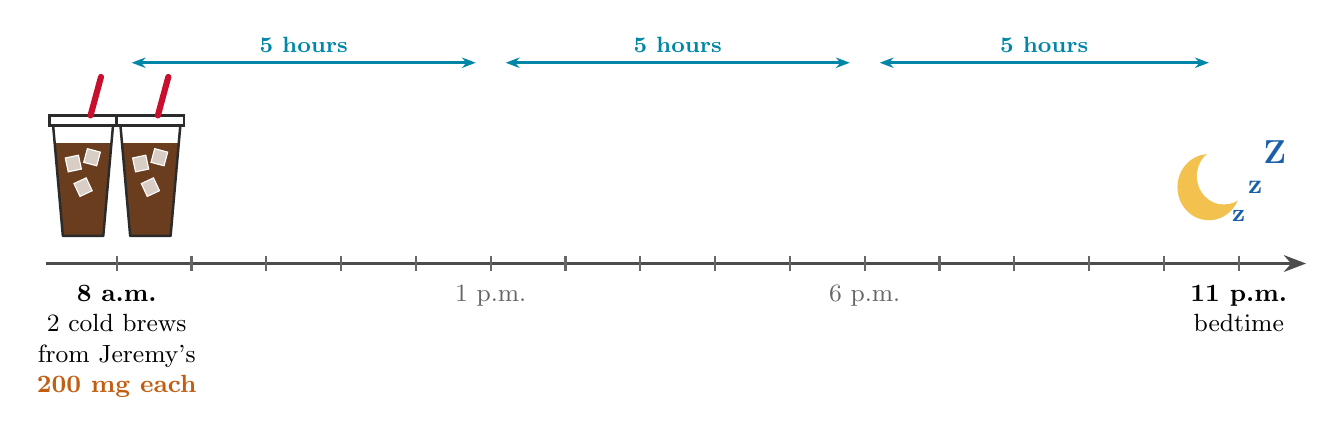
\begin{tikzpicture}[x=0.95cm, y=1cm]
  \draw[black!70, line width=1.4pt, -{Stealth[length=8pt]}] (-0.95,0) -- (15.9,0);
  \foreach \h in {0,...,15} \draw[black!60, line width=0.8pt] (\h,-0.1) -- (\h,0.1);
  % 8 a.m.
  \pic at (-0.45,0.35) {coldbrew};
  \pic at (0.45,0.35) {coldbrew};
  \node[below, align=center, font=\small] at (0,-0.15)
    {\textbf{8~a.m.}\\2 cold brews\\from Jeremy's\\
     {\color{cborange}\bfseries 200 mg each}};
  % the half-life marks
  \node[below, font=\small, text=black!60] at (5,-0.15) {1~p.m.};
  \node[below, font=\small, text=black!60] at (10,-0.15) {6~p.m.};
  % 11 p.m.
  \pic at (14.6,0.35) {bedtime};
  \node[below, align=center, font=\small] at (15,-0.15)
    {\textbf{11~p.m.}\\bedtime};
  % three half-lives
  \foreach \a/\b in {0.2/4.8, 5.2/9.8, 10.2/14.6}
    \draw[cbteal, line width=0.9pt, {Stealth[length=5pt]}-{Stealth[length=5pt]}]
      (\a,2.55) -- node[above, font=\footnotesize\bfseries, text=cbteal] {5 hours} (\b,2.55);
\end{tikzpicture}
\end{center}

\begin{wordhelp}
  \renewcommand{\arraystretch}{1.15}
  \begin{tabularx}{\linewidth}{@{}W{2.9cm} L@{}}
    caffeine & a chemical in coffee, tea, cola and energy drinks. It keeps you
      awake.\frin{la caf\'eine~: une substance chimique du caf\'e, du th\'e, du
      cola et des boissons \'energisantes. Elle te tient \'eveill\'e.} \\
    mg & milligram. A grain of rice is about 20 mg.\frin{le milligramme. Un
      grain de riz p\`ese environ 20~mg.} \\
    cold brew & strong coffee made slowly with cold water\frin{un caf\'e fort,
      infus\'e lentement dans de l'eau froide} \\
    halve & cut in half: divide by 2\frin{couper en deux~: diviser par 2} \\
    curve & a line that bends smoothly\frin{une courbe~: une ligne arrondie,
      sans angle} \\
  \end{tabularx}
\end{wordhelp}

\qhead{A1}{Halving\frin{Diviser par 2}}
\noindent\begin{minipage}{\linewidth}
\noindent Halve each number.
\fr{Divise chaque nombre par 2 (\eng{halve}), case apr\`es case.}

\vspace{6pt}
\begin{center}
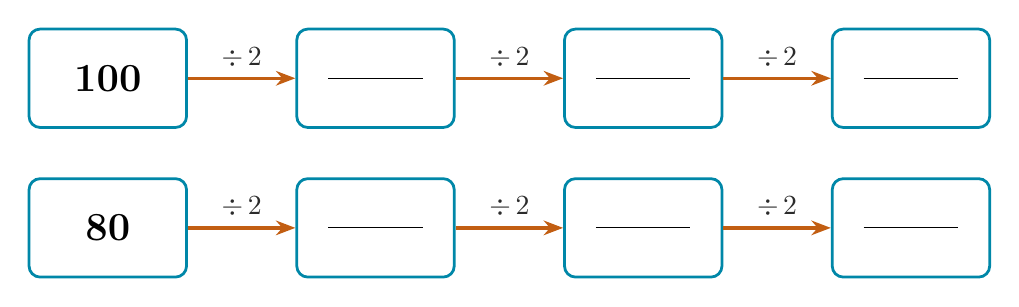
\begin{tikzpicture}[x=1cm, y=1cm]
  \tikzset{hbox/.style={cbox, minimum width=2.0cm, minimum height=1.25cm}}
  \node[hbox] (a0) at (0,0)   {\Large\bfseries 100};
  \node[hbox] (a1) at (3.4,0) {\rule{1.2cm}{0.4pt}};
  \node[hbox] (a2) at (6.8,0) {\rule{1.2cm}{0.4pt}};
  \node[hbox] (a3) at (10.2,0) {\rule{1.2cm}{0.4pt}};
  \node[hbox] (b0) at (0,-1.9)   {\Large\bfseries 80};
  \node[hbox] (b1) at (3.4,-1.9) {\rule{1.2cm}{0.4pt}};
  \node[hbox] (b2) at (6.8,-1.9) {\rule{1.2cm}{0.4pt}};
  \node[hbox] (b3) at (10.2,-1.9) {\rule{1.2cm}{0.4pt}};
  \foreach \r in {a,b}
    \foreach \i/\j in {0/1,1/2,2/3}
      \draw[chainarrow] (\r\i.east) -- node[above, font=\bfseries, text=ink]
        {$\div\,2$} (\r\j.west);
\end{tikzpicture}
\end{center}
\end{minipage}

\qhead{A2}{Mr Bowen's caffeine\frin{La caf\'eine de Mr Bowen}}
\noindent\begin{minipage}{\linewidth}
\noindent (a) Two cold brews: \ $2 \times 200 =$ \mg
\fr{(a) Deux \eng{cold brews} de 200~mg chacun~: combien de caf\'eine en
tout~?}

\vspace{10pt}
\noindent (b) Fill in the boxes. Every 5 hours, \textbf{halve} the caffeine.
\fr{(b) Compl\`ete les cases. Toutes les 5 heures, divise la caf\'eine par 2
(\eng{halve}).}

\vspace{8pt}
\begin{center}
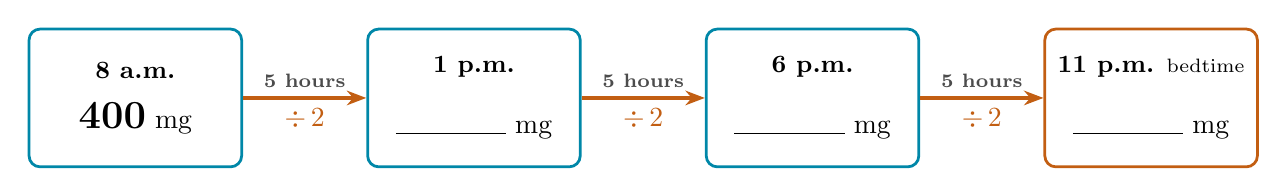
\begin{tikzpicture}[x=1cm, y=1cm]
  \tikzset{tbox/.style={cbox, minimum width=2.7cm, minimum height=1.75cm}}
  \node[tbox] (c0) at (0,0)
    {\textbf{\small 8~a.m.}\\[6pt]{\Large\bfseries 400} mg};
  \node[tbox] (c1) at (4.3,0)
    {\textbf{\small 1~p.m.}\\[10pt]\rule{1.4cm}{0.4pt} mg};
  \node[tbox] (c2) at (8.6,0)
    {\textbf{\small 6~p.m.}\\[10pt]\rule{1.4cm}{0.4pt} mg};
  \node[tbox, draw=cborange] (c3) at (12.9,0)
    {\textbf{\small 11~p.m.} {\scriptsize bedtime}\\[10pt]\rule{1.4cm}{0.4pt} mg};
  \foreach \i/\j in {0/1,1/2,2/3}
    \draw[chainarrow] (c\i.east) -- node[above, font=\scriptsize\bfseries, text=black!70]
      {5 hours} node[below, font=\bfseries] {$\div\,2$} (c\j.west);
\end{tikzpicture}
\end{center}
\end{minipage}

\qhead{A3}{Does it ever run out?\frin{La caf\'eine finit-elle par dispara\^itre~?}}
\noindent\begin{minipage}{\linewidth}
\noindent (a) Keep halving after bedtime.
\fr{(a) Continue \`a diviser par 2 apr\`es l'heure du coucher (\eng{bedtime}).}

\vspace{6pt}
\begin{center}
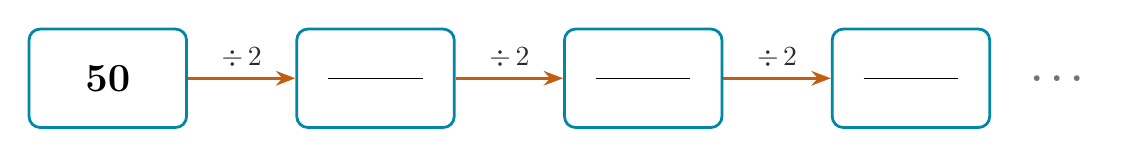
\begin{tikzpicture}[x=1cm, y=1cm]
  \tikzset{hbox/.style={cbox, minimum width=2.0cm, minimum height=1.25cm}}
  \node[hbox] (d0) at (0,0)   {\Large\bfseries 50};
  \node[hbox] (d1) at (3.4,0) {\rule{1.2cm}{0.4pt}};
  \node[hbox] (d2) at (6.8,0) {\rule{1.2cm}{0.4pt}};
  \node[hbox] (d3) at (10.2,0) {\rule{1.2cm}{0.4pt}};
  \foreach \i/\j in {0/1,1/2,2/3}
    \draw[chainarrow] (d\i.east) -- node[above, font=\bfseries, text=ink]
      {$\div\,2$} (d\j.west);
  \node[font=\Large\bfseries, text=black!55] at (12.1,0) {\ldots};
\end{tikzpicture}
\end{center}

\vspace{4pt}
\noindent (b) If you keep halving, does the number ever get to 0? \hfill
\choice{yes} \quad\; \choice{no}
\fr{(b) Si tu continues \`a diviser par 2, est-ce que le nombre finit par
arriver \`a 0~?}
\end{minipage}

\vspace{12pt}
\noindent\begin{minipage}{\linewidth}
\noindent (c) Fill in the gap with one word from the box.
\fr{(c) Compl\`ete la phrase avec un mot de l'encadr\'e.}

\vspace{4pt}
\begin{center}
\fbox{\rule[-0.4em]{0pt}{1.5em}\ half-life \qquad limitation \qquad molecule\ }
% Inside the centre, not after it: \fr's \unskip would eat the space below.
\fr{\eng{half-life} = la demi-vie \sep \eng{limitation} = une limite \sep
\eng{molecule} = une mol\'ecule}
\end{center}

\vspace{2pt}
\noindent The maths model says the caffeine \textbf{never} runs out. But real
caffeine is made of molecules, and the last one is gone after about
\textbf{2 weeks}. So the model is wrong here.
\fr{Le mod\`ele math\'ematique dit que la caf\'eine ne dispara\^it
\textbf{jamais}. Mais la vraie caf\'eine est faite de mol\'ecules, et la
derni\`ere a disparu au bout d'environ \textbf{2 semaines}. Ici, le mod\`ele se
trompe donc.}

\vspace{8pt}
\noindent This is a \blank[4.0cm] of the model.
\fr{C'est une \ldots\ du mod\`ele. \'Ecris le mot en anglais.}
\end{minipage}

% ---------------------------------------------------------------------------
\qhead{A4}{Draw the graph\frin{Trace le graphique}}
\noindent\begin{minipage}{\linewidth}
\noindent Put a dot for every box in A2. The first part is drawn for you. Join
the dots with a \textbf{smooth curve}, not straight lines.
\fr{Place un point pour chaque case de A2. Le d\'ebut est d\'ej\`a trac\'e.
Relie les points par une \textbf{courbe} bien arrondie (\eng{smooth curve}),
pas par des traits droits.}

\vspace{6pt}
\begin{center}
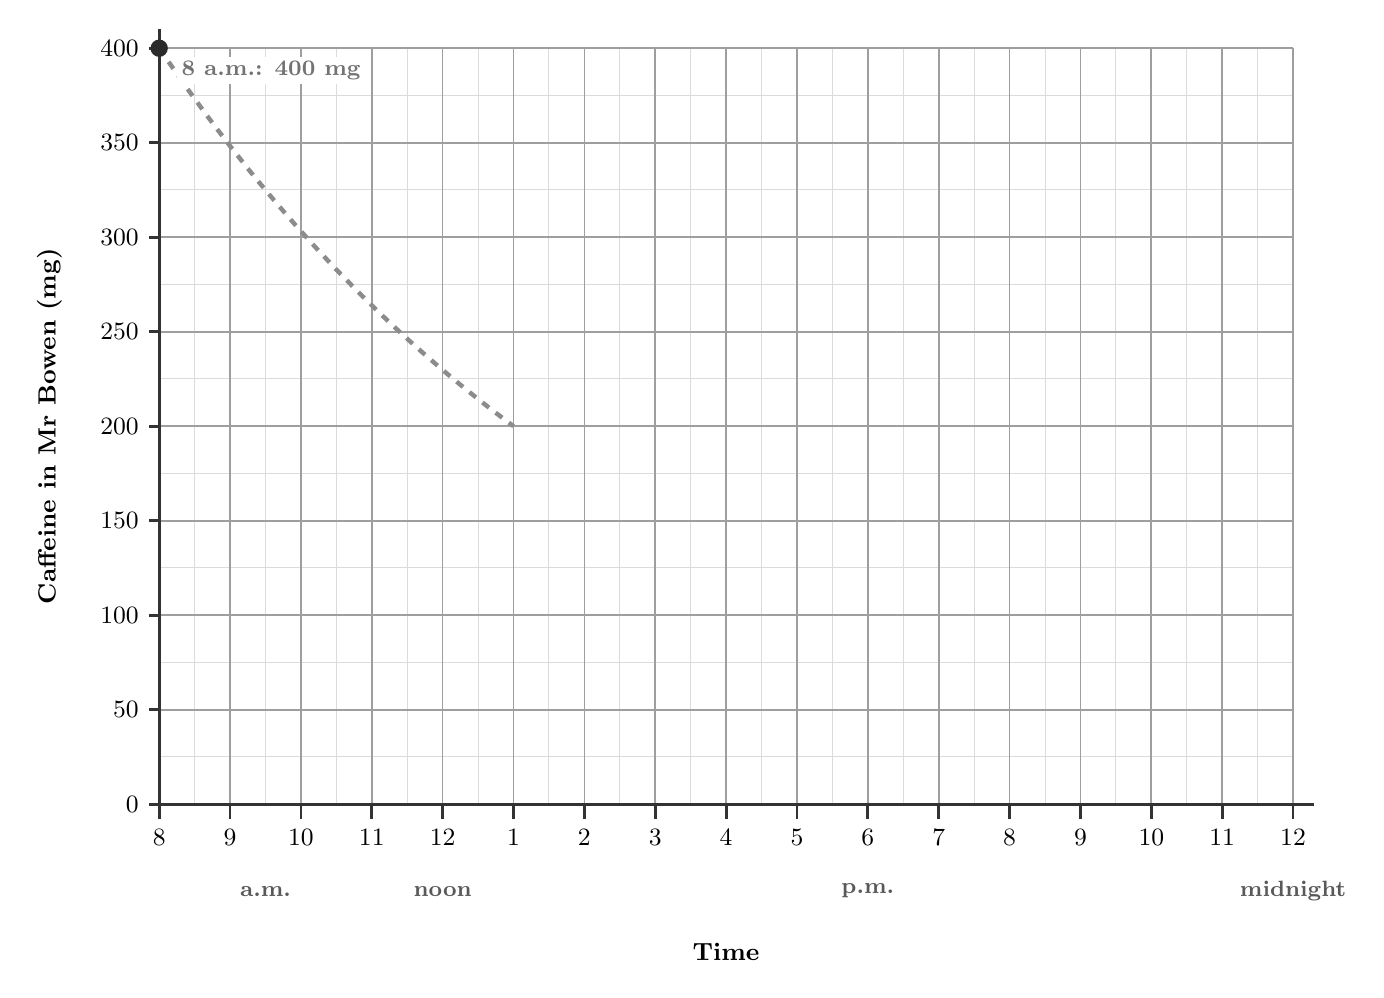
\begin{tikzpicture}[x=0.9cm, y=\agraphy]
  \bowenaxes
  \draw[black!45, line width=1.6pt, dashed] plot[domain=0:5, samples=40, smooth]
    (\x, {400*0.5^(\x/5)});
  \fill[ink] (0,400) circle (0.11cm);
  \node[right, font=\footnotesize\bfseries, text=black!55, fill=white,
        inner sep=1.5pt] at (0.25,388) {8~a.m.: 400 mg};
\end{tikzpicture}
\end{center}
\end{minipage}

\qhead{A5}{Read the graph\frin{Lis le graphique}}
\noindent Mr Bowen marks your homework at \textbf{8~p.m.}
\fr{Mr Bowen corrige tes devoirs \`a 8~h du soir (\eng{8 p.m.}).}

\vspace{8pt}
\noindent (a) 8~p.m. is between 6~p.m. and 11~p.m. So his caffeine is between
\mg[1.4cm] and \mg[1.4cm].
\fr{(a) 8~h du soir, c'est entre 6~h et 11~h du soir. Il a donc entre \ldots\
mg et \ldots\ mg de caf\'eine.}

\vspace{10pt}
\noindent (b) Go \textbf{up} from 8~p.m. to your curve, then \textbf{across}.
How much caffeine is in him at 8~p.m.? \quad about \mg
\fr{(b) Pars de 8~h du soir et monte (\eng{up}) jusqu'\`a ta courbe, puis va
\`a l'horizontale (\eng{across}) jusqu'\`a l'axe. Combien de caf\'eine a-t-il
dans le corps \`a 8~h du soir~?}

\qhead{A6}{The title question\frin{La question du titre}}
% One block in the French copy: the question, its starter and its lines go
% over a page together (the lines were left behind once).
\iffr\noindent\begin{minipage}{\linewidth}\fi
\noindent Why is Mr Bowen still awake at 11~p.m.? Use your number from A2.
A cup of coffee has about 100 mg. How much coffee is that?
\fr{Pourquoi Mr Bowen ne dort-il toujours pas \`a 11~h du soir~? Utilise ton
r\'esultat de A2. Une tasse de caf\'e contient environ 100~mg~: \c{c}a fait
combien de caf\'e~? R\'eponds en anglais.}

\vspace{4pt}
\noindent\starter{Mr Bowen is still awake because at 11~p.m. he still has
\ldots}
\qlines{\frl{4}{6}}
\iffr\end{minipage}\fi

% ===========================================================================
% PART B -- THE INTERVIEW
% ===========================================================================
\hwsection{Part B\quad Interview a Caffeine Drinker\frin{Interviewe quelqu'un
qui boit de la caf\'eine}}

\begin{activity}[What you will do\frin{Ce que tu vas faire}]
  \noindent \textbf{Interview} an adult in your family who drinks coffee, tea,
  cola or energy drinks like Sting. Then work out how much caffeine is in
  their body at \textbf{bedtime}.
  \fr{Interviewe un adulte de ta famille qui boit du caf\'e, du th\'e, du cola
  ou des boissons \'energisantes comme le Sting. Ensuite, calcule combien de
  caf\'eine il reste dans son corps au moment du coucher (\eng{bedtime}).}

  \vspace{4pt}
  \noindent You can do the interview in \textbf{any language}. Write in
  \textbf{English}.
  \fr{Tu peux faire l'interview dans la langue que tu veux. \'Ecris tes
  r\'eponses \textbf{en anglais}.}
\end{activity}

\begin{wordhelp}
  \renewcommand{\arraystretch}{1.15}
  \begin{tabularx}{\linewidth}{@{}W{2.9cm} L@{}}
    interview & ask someone questions, and write down the answers\frin{interviewer~:
      poser des questions \`a quelqu'un et noter ses r\'eponses} \\
    label & the words printed on a can or bottle. They say what is
      inside.\frin{l'\'etiquette~: ce qui est \'ecrit sur la canette ou la
      bouteille. Elle dit ce qu'il y a dedans.} \\
    search & type words into Google to find something\frin{chercher~: taper
      des mots dans Google pour trouver quelque chose} \\
    estimate & a careful guess, using numbers\frin{une estimation~: une
      supposition r\'efl\'echie, faite avec des nombres} \\
  \end{tabularx}
\end{wordhelp}

\qhead{B1}{The interview\frin{L'interview}}
% One block in the French copy: it split the list mid-question.
\iffr\noindent\begin{minipage}{\linewidth}\fi
\noindent Ask about \textbf{yesterday}.
\fr{Pose tes questions sur la journ\'ee d'\textbf{hier} (\eng{yesterday}).}

\begin{enumerate}[label=\textbf{\arabic*.}, itemsep=2pt, topsep=4pt]
  \item ``Can I interview you for my homework?''
    \fr{\fq{Est-ce que je peux t'interviewer pour mes devoirs~?}}
  \item ``What was your \textbf{first} drink with caffeine yesterday? How big
    was it?''\newline {\small\color{black!60}For example: 1 can of Sting,
    330 ml.}
    \fr{\fq{Quelle a \'et\'e ta \textbf{premi\`ere} boisson avec de la
    caf\'eine hier~? Elle faisait quelle taille~?} Par exemple~: une canette de
    Sting, 330~ml.}
  \item ``What time did you drink it?''
    \fr{\fq{Tu l'as bue \`a quelle heure~?}}
  \item ``What time did you go to bed?''
    \fr{\fq{Tu t'es couch\'e(e) \`a quelle heure~?}}
\end{enumerate}
\iffr\end{minipage}\fi

\vspace{2pt}
\noindent\begin{minipage}{\linewidth}
\renewcommand{\arraystretch}{2.0}
\noindent\begin{tabularx}{\linewidth}{@{}l X@{}}
  \textbf{I interviewed my} & \blank[5.0cm]\,. \\
  \textbf{Their first drink was} & \blank[10.5cm] \\
  \textbf{They drank it at} & \blank[4.0cm]\,. \\
  \textbf{They went to bed at} & \blank[4.0cm]\,. \\
\end{tabularx}
\fr{Compl\`ete en anglais~: qui tu as interview\'e (\eng{my mother},
\eng{my uncle}\ldots), sa boisson, l'heure o\`u il ou elle l'a bue et l'heure
du coucher.}
\end{minipage}

% ---------------------------------------------------------------------------
\qhead{B2}{Find the caffeine\frin{Trouve la quantit\'e de caf\'eine}}

\begin{activity}[Where to look\frin{O\`u chercher}]
  \begin{minipage}[t]{0.68\linewidth}
    \begin{enumerate}[label=\textbf{\arabic*.}, itemsep=3pt, topsep=0pt]
      \item \textbf{The label} on the can or bottle. Look for the word
        \textbf{caffeine}.
        \fr{L'\'etiquette (\eng{label}) de la canette ou de la bouteille.
        Cherche le mot \eng{caffeine}.}
      \item \textbf{Google.} Search for the drink, like this: \\
        \textit{caffeine in 1 can of Sting mg}
        \fr{Google. Tape le nom de la boisson, comme dans cet exemple.}
    \end{enumerate}

    \vspace{5pt}
    \noindent Milk, sugar and ice: \key{0 mg}.
    \fr{Le lait, le sucre et les gla\c{c}ons~: 0~mg.}

    \vspace{3pt}
    \noindent Two numbers, like 50 to 80 mg? Use the \textbf{middle}: 65 mg.
    \fr{Deux nombres, comme \fq{50 to 80 mg}~? Prends celui du milieu
    (\mbox{\eng{middle}})~: 65~mg.}
  \end{minipage}\hfill
  \begin{minipage}[t]{0.28\linewidth}\vspace{-6pt}\centering
    % A bottle with its label. No real brand: the numbers are made up.
    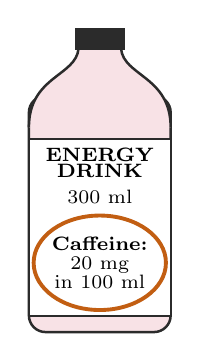
\begin{tikzpicture}[x=1cm, y=1cm]
      \draw[ink, line width=0.9pt, fill=cbred!12, rounded corners=6pt]
        (-0.9,0) rectangle (0.9,3.0);
      \draw[ink, line width=0.9pt, fill=cbred!12]
        (-0.9,2.6) .. controls (-0.9,3.25) and (-0.3,3.25) .. (-0.27,3.6) --
        (0.27,3.6) .. controls (0.3,3.25) and (0.9,3.25) .. (0.9,2.6);
      \draw[ink, line width=0.9pt, fill=ink] (-0.3,3.6) rectangle (0.3,3.85);
      \draw[ink, line width=0.6pt, fill=white] (-0.9,0.2) rectangle (0.9,2.45);
      \node[font=\scriptsize\bfseries, align=center] at (0,2.15) {ENERGY\\[-2pt]DRINK};
      \node[font=\scriptsize] at (0,1.72) {300 ml};
      \node[font=\scriptsize, align=center] at (0,0.88)
        {\textbf{Caffeine:}\\[-1pt]20 mg\\[-1pt]in 100 ml};
      \draw[cborange, line width=1.4pt] (0,0.88) ellipse (0.84cm and 0.6cm);
    \end{tikzpicture}
  \end{minipage}
\end{activity}

\noindent\begin{minipage}{\linewidth}
\noindent\textbf{Some labels give the caffeine in 100 ml.} This bottle has
20 mg in every 100 ml. It holds 300~ml.
\fr{Certaines \'etiquettes donnent la caf\'eine pour 100~ml. Cette bouteille
contient 20~mg pour 100~ml, et elle fait 300~ml en tout.}

\vspace{3pt}
\noindent 300 ml is 3 lots of 100 ml. \qquad $3 \times 20 =$ \key{60 mg} in the
whole bottle.
\fr{300~ml, c'est 3 fois 100~ml (\eng{3 lots of 100 ml})~: il y a donc 60~mg
dans toute la bouteille.}

\vspace{3pt}
\noindent{\small\color{black!65} A 330 ml can? \ $330 \div 100 = 3.3$, then
$3.3 \times 20 = 66$ mg. Or search on Google for the whole can.}
\fr{Une canette de 330~ml~? Fais $330 \div 100 = 3.3$, puis
$3.3 \times 20 = 66$~mg. Ou cherche sur Google la caf\'eine de toute la
canette.}

\vspace{12pt}
\noindent Their drink has about \mg[2.2cm] of caffeine.
\fr{Sa boisson contient environ \ldots\ mg de caf\'eine.}

\vspace{10pt}
\noindent I found it on: \quad \choice{the label} \quad\;
\choice{Google} \quad\; \choice{another website}
\fr{Je l'ai trouv\'e sur~: l'\'etiquette, Google ou un autre site web.}
\end{minipage}

% ---------------------------------------------------------------------------
\qhead{B3}{Halve it, every 5 hours\frin{Divise par 2 toutes les 5 heures}}
\noindent\begin{minipage}{\linewidth}
\noindent Start with their drink. In each box, \textbf{add 5 hours} to the
time and \textbf{halve} the caffeine. Keep going until you are
\textbf{past their bedtime}.
\fr{Commence par sa boisson. \`A chaque case, ajoute 5 heures (\eng{add 5
hours}) et divise la caf\'eine par 2 (\eng{halve}). Continue jusqu'\`a
d\'epasser l'heure de son coucher (\eng{past their bedtime}).}

\vspace{8pt}
\noindent{\small\bfseries\color{black!60}Example: a cup of tea, about 40 mg,
at 7~a.m.}
\fr{Exemple~: une tasse de th\'e, environ 40~mg, \`a 7~h du matin. \eng{The
drink} = la boisson \sep \eng{5 hours later} = 5 heures plus tard \sep
\eng{Time} = l'heure}

\vspace{3pt}
{\renewcommand{\arraystretch}{1.25}%
\noindent\begin{tabular}{|p{2.45cm}|C{2.3cm}|C{2.3cm}|C{2.3cm}|C{2.3cm}|C{2.3cm}|}
  \halvehead
  \textbf{Time} & \starter{7~a.m.} & \starter{12 noon} & \starter{5~p.m.} &
    \starter{10~p.m.} & \starter{3~a.m.} \\ \hline
  \textbf{Caffeine (mg)} & \starter{40} & \starter{20} & \starter{10} &
    \starter{5} & \starter{2.5} \\ \hline
\end{tabular}}

\vspace{12pt}
\noindent{\small\bfseries\color{cbteal}Now yours:\frin{\`A toi~:}}

\vspace{3pt}
\noindent\begin{tabular}{|p{2.45cm}|C{2.3cm}|C{2.3cm}|C{2.3cm}|C{2.3cm}|C{2.3cm}|}
  \halvehead
  \textbf{Time}\tall & & & & & \\ \hline
  \textbf{Caffeine (mg)}\tall & & & & & \\ \hline
\end{tabular}
\end{minipage}

\qhead{B4}{Bedtime\frin{L'heure du coucher}}
\noindent (a) Their bedtime is between the times in two of your boxes:
\blank[2.6cm] and \blank[2.6cm].
\fr{(a) L'heure du coucher se situe entre les heures de deux de tes cases~:
lesquelles~?}

\vspace{10pt}
\noindent (b) So at bedtime, they have between \mg[1.6cm] and \mg[1.6cm].
\fr{(b) Donc, au moment du coucher, la personne a entre \ldots\ mg et \ldots\
mg de caf\'eine.}

\vspace{10pt}
\noindent (c) Choose a number in between. At bedtime, they have about
\mg[1.8cm] of caffeine.
\fr{(c) Choisis un nombre entre les deux. Au coucher, la personne a environ
\ldots\ mg de caf\'eine.}

\qhead{B5}{Compare with Mr Bowen\frin{Compare avec Mr Bowen}}
% One block in the French copy, like A6.
\iffr\noindent\begin{minipage}{\linewidth}\fi
\noindent Mr Bowen had 50 mg at bedtime. Did your adult have
\textbf{more} or \textbf{less}? Why? Think about how \textbf{big} the drink
was, and \textbf{what time} they drank it.
\fr{Mr Bowen avait 50~mg au coucher. Et la personne que tu as interview\'ee~:
plus (\eng{more}) ou moins (\eng{less})~? Pourquoi~? Pense \`a la taille de la
boisson et \`a l'heure o\`u elle a \'et\'e bue. R\'eponds en anglais.}

\vspace{4pt}
\noindent\starter{At bedtime my \blank[2.4cm] had about \blank[1.4cm] mg of
caffeine. That is more / less than Mr Bowen, because \ldots}
\qlines{\frl{4}{6}}
\iffr\end{minipage}\fi

\qhead{B6}{Is your number right?\frin{Ton nombre est-il juste~?}}
\noindent\begin{minipage}{\linewidth}
\noindent Your bedtime number is an \textbf{estimate}. Tick \textbf{one}
reason it might be wrong. Then write it as a sentence.
\fr{Ton nombre au coucher est une estimation (\eng{estimate}). Coche
\textbf{une} raison pour laquelle il pourrait \^etre faux, puis \'ecris-la en
une phrase, en anglais.}

\vspace{6pt}
\renewcommand{\arraystretch}{1.6}
\begin{tabularx}{\linewidth}{@{}p{0.8cm}L@{}}
  \tickbox & They had other drinks with caffeine too.\frin{La personne a bu
    d'autres boissons avec de la caf\'eine.} \\
  \tickbox & Caffeine's half-life is not 5 hours for everybody.\frin{La
    demi-vie de la caf\'eine n'est pas de 5 heures pour tout le monde.} \\
  \tickbox & The number from the label or Google may not be exact.\frin{Le
    nombre de l'\'etiquette ou de Google n'est peut-\^etre pas exact.} \\
\end{tabularx}

\vspace{2pt}
\noindent\starter{My bedtime number might be wrong because \ldots}
\wlines{\frl{3}{5}}
\end{minipage}

% ===========================================================================
% PART C -- CARBON DATING
% ===========================================================================
\hwsection{Part C\quad Carbon Dating\frin{La datation au carbone 14}}
\qhead{C1}{The halving chain\frin{La cha\^ine des moiti\'es}}
\noindent\begin{minipage}{\linewidth}
\noindent Caffeine halves every 5 hours. Carbon-14 halves every
\textbf{5\,700 years}. Fill in the boxes.
\fr{La caf\'eine diminue de moiti\'e toutes les 5 heures. Le carbone 14
diminue de moiti\'e tous les \textbf{5\,700 ans}. Compl\`ete les cases.}

\vspace{8pt}
\begin{center}
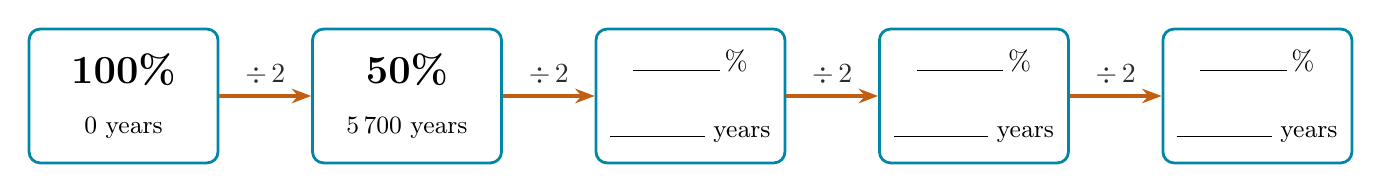
\begin{tikzpicture}[x=1cm, y=1cm]
  \tikzset{kbox/.style={cbox, minimum width=2.4cm, minimum height=1.7cm}}
  \node[kbox] (k0) at (0,0)    {{\Large\bfseries 100\%}\\[6pt]{\small 0 years}};
  \node[kbox] (k1) at (3.6,0)  {{\Large\bfseries 50\%}\\[6pt]{\small 5\,700 years}};
  \node[kbox] (k2) at (7.2,0)  {\rule{1.1cm}{0.4pt}\,\%\\[12pt]{\small\rule{1.2cm}{0.4pt} years}};
  \node[kbox] (k3) at (10.8,0) {\rule{1.1cm}{0.4pt}\,\%\\[12pt]{\small\rule{1.2cm}{0.4pt} years}};
  \node[kbox] (k4) at (14.4,0) {\rule{1.1cm}{0.4pt}\,\%\\[12pt]{\small\rule{1.2cm}{0.4pt} years}};
  \foreach \i/\j in {0/1,1/2,2/3,3/4}
    \draw[chainarrow] (k\i.east) -- node[above, font=\bfseries, text=ink]
      {$\div\,2$} (k\j.west);
\end{tikzpicture}
\end{center}

\vspace{2pt}
\noindent{\small\color{black!65}Each box is 5\,700 years more than the one
before it.}
\fr{Chaque case a 5\,700 ans de plus que la pr\'ec\'edente.}
\end{minipage}

% ---------------------------------------------------------------------------
\qhead{C2}{The museum\frin{Le mus\'ee}}
\noindent\begin{minipage}{\linewidth}
\noindent Scientists measured the carbon-14 left in five objects. Use C1.
\fr{Des scientifiques ont mesur\'e le carbone 14 qui reste dans cinq objets.
Utilise C1.}

\vspace{4pt}
\noindent\textbf{Careful:} carbon dating only works for things that were
\key{alive}, up to about \key{50\,000 years} old. If it does not work, write
\textbf{does not work}.
\fr{Attention~: la datation au carbone 14 ne marche que pour ce qui a \'et\'e
vivant (\eng{alive}), jusqu'\`a environ 50\,000 ans. Si elle ne marche pas,
\'ecris \eng{does not work}.}

\vspace{6pt}
\renewcommand{\arraystretch}{1.2}
\noindent\begin{tabularx}{\linewidth}{|L|C{2.2cm}|C{2.2cm}|C{2.3cm}|C{3.3cm}|}
  \hline
  \hrow \textbf{Object}\frin{l'objet} & \textbf{Was it ever alive?}\frin{A-t-il
    \'et\'e vivant~?} & \textbf{Carbon-14 left}\frin{carbone 14 restant} &
    \textbf{How many half-lives?}\frin{combien de demi-vies~?} &
    \textbf{Age (years)}\frin{\^age en ann\'ees} \\ \hline
  \starter{A wooden boat}\frcell{un bateau en bois}\ctall & \starter{yes} &
    \starter{50\%} & \starter{1} & \starter{5\,700} \\ \hline
  A bear bone from a cave\frcell{un os d'ours trouv\'e dans une grotte}\ctall &
    & 25\% & & \\ \hline
  A wooden spear\frcell{une lance en bois}\ctall & & 12.5\% & & \\ \hline
  A stone axe\frcell{une hache en pierre}\ctall & & --- & & \\ \hline
  A \textit{T.\ rex} tooth\frcell{une dent de \textit{T.\ rex}}\ctall & & 0\% &
    & \\ \hline
\end{tabularx}

\vspace{3pt}
\noindent{\small\color{cbblue}\textbf{Word help:} a \textbf{spear} is a long
stick with a sharp point \sep an \textbf{axe} is a tool for cutting wood \sep
a \textbf{\textit{T.\ rex}} is a dinosaur}
\fr{Une lance (\eng{spear}) est un long b\^aton pointu \sep une hache
(\eng{axe}) sert \`a couper le bois \sep le \textit{T.\ rex} est un dinosaure}
\end{minipage}

\qhead{C3}{Why does it not work?\frin{Pourquoi \c{c}a ne marche pas~?}}
\noindent (a) Carbon dating does not work for the stone axe, because stone
was never \blank[3.2cm]\,.
\fr{(a) La datation au carbone 14 ne marche pas pour la hache en pierre, parce
que la pierre n'a jamais \'et\'e \ldots\ (\'ecris le mot en anglais).}

\vspace{12pt}
\noindent (b) Carbon dating does not work for the \textit{T.\ rex} tooth,
because it is too \blank[3.2cm]\,.
\fr{(b) Elle ne marche pas non plus pour la dent de \textit{T.\ rex}, parce
qu'elle est trop \ldots}

\vspace{2pt}
\noindent{\small\color{black!65}\textit{Clue:} dinosaurs died out about
66 million years ago.}
\fr{Indice~: les dinosaures ont disparu il y a environ 66 millions
d'ann\'ees.}

% ===========================================================================
% PART D -- THE SUN
% ===========================================================================
% A new page in the French copy, so it lands on 14 pages for certain: D1 and
% D2 do not fit on one page there, and D2 takes the next one to itself.
\iffr\clearpage\fi
\hwsection{Part D\quad The Sun: Different Speeds, the Same Maths\frin{Le
Soleil~: des vitesses diff\'erentes, les m\^emes maths}}

\begin{remember}
  \key{Caffeine}, \key{carbon-14} and the \key{Sun's hydrogen} all disappear
  at a rate we can model with maths. Measure what is \key{left} to find
  \key{how long} it has been.
  \fr{La caf\'eine, le carbone 14 et l'hydrog\`ene du Soleil disparaissent
  tous \`a un rythme qu'on peut d\'ecrire avec des maths. Mesure ce qui reste
  (\eng{left}) pour savoir combien de temps s'est \'ecoul\'e (\eng{how long}).}
\end{remember}

\vspace{2pt}
\noindent{\small\color{cbblue}\textbf{Word help:} the \textbf{core} is the
middle of the Sun \sep \textbf{hydrogen} and \textbf{helium} are gases \sep
a \textbf{billion} is a thousand million}
\fr{Le c\oe{}ur (\eng{core}) est le centre du Soleil \sep l'hydrog\`ene
(\eng{hydrogen}) et l'h\'elium (\eng{helium}) sont des gaz \sep attention~: un
\eng{billion} en anglais, c'est un \textbf{milliard} en fran\c{c}ais (mille
millions)}

\qhead{D1}{How old is the Sun?\frin{Quel \^age a le Soleil~?}}
\noindent Nobody can take a piece of the Sun. So scientists build a
\textbf{model Sun} with maths, and let it get older until it matches the real
Sun.
\fr{Personne ne peut aller chercher un morceau du Soleil. Alors les
scientifiques construisent un Soleil mod\`ele (\eng{model Sun}) avec des
maths, et le font vieillir jusqu'\`a ce qu'il ressemble au vrai Soleil.}

\vspace{10pt}
\noindent (a) The Sun turns \blank[3.0cm] into \blank[3.0cm]\,.
\fr{(a) Le Soleil transforme \ldots\ en \ldots\ (\'ecris les mots en
anglais).}

\vspace{10pt}
\noindent (b) When the Sun was born, its core was \textbf{71\%} hydrogen.
Half of 71\% is \blank[2.0cm]\,\%.
\fr{(b) \`A la naissance du Soleil, son c\oe{}ur contenait 71\,\%
d'hydrog\`ene. Combien fait la moiti\'e de 71\,\%~?}

\vspace{10pt}
\noindent (c) Today the core is \textbf{34\%} hydrogen. Is about
\textbf{half} of the hydrogen gone? \hfill \choice{yes} \quad\; \choice{no}
\fr{(c) Aujourd'hui, le c\oe{}ur contient 34\,\% d'hydrog\`ene. Est-ce
qu'environ la moiti\'e de l'hydrog\`ene a disparu~?}

\vspace{10pt}
\noindent (d) The model Sun matches the real Sun at about \blank[1.6cm]
billion years. So the Sun is about \blank[1.6cm] billion years old.
\fr{(d) Le Soleil mod\`ele ressemble au vrai Soleil vers \ldots\ milliards
d'ann\'ees (\eng{billion years}). Le Soleil a donc environ \ldots\ milliards
d'ann\'ees.}

\qhead{D2}{Three clocks\frin{Trois horloges}}
\noindent\begin{minipage}{\linewidth}
\noindent Draw a line from each clock to how fast it goes.
\fr{Relie chaque horloge \`a sa vitesse.}

\vspace{8pt}
\begin{center}
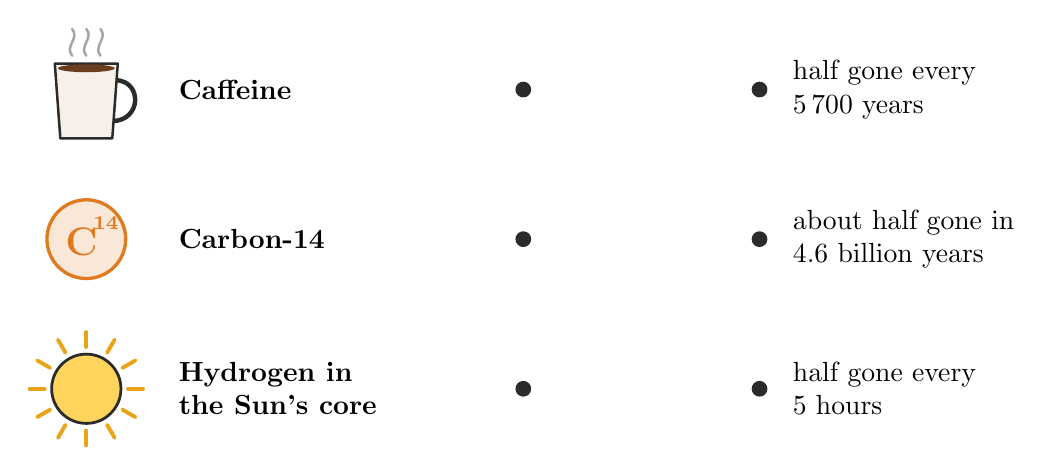
\begin{tikzpicture}[x=1cm, y=1cm]
  \pic at (0.45,-0.62) {mug};
  \node[right, font=\bfseries] at (1.5,0) {Caffeine};
  \pic at (0.45,\dtwoB) {cfourteen};
  \node[right, font=\bfseries] at (1.5,\dtwoB) {Carbon-14};
  \pic at (0.45,\dtwoC) {sun};
  \node[right, font=\bfseries, align=left] at (1.5,\dtwoC)
    {Hydrogen in\\the Sun's core\frnode{l'hydrog\`ene}\frnode{au c\oe{}ur du
    Soleil}};
  \foreach \y in {0,\dtwoB,\dtwoC} \fill[ink] (6.0,\y) circle (0.1);
  \foreach \y in {0,\dtwoB,\dtwoC} \fill[ink] (9.0,\y) circle (0.1);
  \node[right, align=left] at (9.3,0) {half gone every\\5\,700 years%
    \frnode{la moiti\'e dispara\^it}\frnode{tous les 5\,700 ans}};
  \node[right, align=left] at (9.3,\dtwoB) {about half gone in\\4.6 billion years%
    \frnode{environ la moiti\'e a disparu}\frnode{en 4.6 milliards
    d'ann\'ees}};
  \node[right, align=left] at (9.3,\dtwoC) {half gone every\\5 hours%
    \frnode{la moiti\'e dispara\^it}\frnode{toutes les 5 heures}};
\end{tikzpicture}
\end{center}

\vspace{6pt}
\noindent Put them in order, \textbf{fastest} first.
\fr{Range-les dans l'ordre, du plus rapide (\eng{fastest}) au plus lent.}

\vspace{8pt}
\noindent 1.\ \blank[4.2cm] \quad 2.\ \blank[4.2cm] \quad 3.\ \blank[4.2cm]
\end{minipage}

% ===========================================================================
% PART E -- CAFFEINE AND SLEEP
% ===========================================================================
% Its own page: the reading, a plan built from the packet's numbers, then the
% letter. Every fact in the guide is in the key with its source.
\clearpage
\hwsection{Part E\quad Caffeine and Sleep\frin{La caf\'eine et le sommeil}}

\begin{remember}[Read this: how caffeine affects sleep\frin{\`A lire~: l'effet de
  la caf\'eine sur le sommeil}]
  \begin{minipage}[t]{0.75\linewidth}
  \begin{enumerate}[label=\textbf{\arabic*.}, itemsep=3pt, topsep=0pt,
                    leftmargin=1.6em]
    \item All day your brain makes \key{adenosine}
      {\small\color{black!60}\mbox{(a-DEN-o-seen)}}, a chemical that makes
      you feel sleepy.
      \fr{Toute la journ\'ee, ton cerveau fabrique de l'ad\'enosine
      (\eng{adenosine}), une substance chimique qui te donne envie de dormir.}
    \item \key{Caffeine blocks adenosine.} The adenosine is still there, but
      your brain cannot feel it.
      \fr{La caf\'eine bloque (\eng{blocks}) l'ad\'enosine. L'ad\'enosine est
      toujours l\`a, mais ton cerveau ne la sent plus.}
    \item Caffeine makes it harder to \textbf{fall asleep} and \textbf{stay
      asleep}.
      \fr{Avec la caf\'eine, on a plus de mal \`a s'endormir (\eng{fall
      asleep}) et \`a rester endormi (\eng{stay asleep}).}
    \item \key{How much is too much?} Even \textbf{100~mg} (one cup of
      coffee) near bedtime can stop an adult sleeping. A child: about
      \textbf{50~mg}.
      \fr{\`A partir de combien, c'est trop~? M\^eme 100~mg (une tasse de
      caf\'e) peu avant le coucher peuvent emp\^echer un adulte de dormir.
      Pour un enfant~: environ 50~mg.}
    \item \key{Stop caffeine 8 hours before bed}, or longer after a big
      drink.
      \fr{Arr\^ete la caf\'eine 8 heures avant d'aller te coucher, et encore
      plus t\^ot apr\`es une grosse boisson.}
    \item At your age you need \textbf{9 to 11 hours} of sleep.
      \fr{\`A ton \^age, tu as besoin de 9 \`a 11 heures de sommeil.}
  \end{enumerate}
  \end{minipage}\hfill
  \begin{minipage}[t]{0.23\linewidth}\vspace{2pt}\centering
    % Caffeine sits in the gaps, so adenosine cannot get in.
    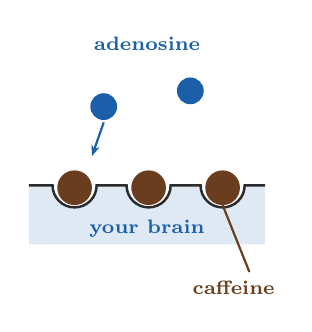
\begin{tikzpicture}[x=1cm, y=1cm]
      \fill[cbblue!14] (0,0) -- (0,0.75) -- (0.3,0.75) arc (180:360:0.28)
        -- (1.24,0.75) arc (180:360:0.28) -- (2.18,0.75) arc (180:360:0.28)
        -- (3.0,0.75) -- (3.0,0) -- cycle;
      \draw[ink, line width=0.9pt] (0,0.75) -- (0.3,0.75) arc (180:360:0.28)
        -- (1.24,0.75) arc (180:360:0.28) -- (2.18,0.75) arc (180:360:0.28)
        -- (3.0,0.75);
      \node[font=\scriptsize\bfseries, text=cbblue] at (1.5,0.2) {your brain};
      \foreach \x in {0.58,1.52,2.46}
        \fill[coffee] (\x,0.72) circle (0.22);
      \fill[cbblue] (0.95,1.75) circle (0.17);
      \fill[cbblue] (2.05,1.95) circle (0.17);
      \draw[cbblue, line width=0.8pt, -{Stealth[length=4pt]}]
        (0.95,1.55) -- (0.8,1.12);
      \node[font=\scriptsize\bfseries, text=cbblue, align=center] at (1.5,2.55)
        {adenosine};
      \draw[coffee, line width=0.8pt] (2.46,0.5) -- (2.8,-0.35);
      \node[font=\scriptsize\bfseries, text=coffee] at (2.6,-0.55) {caffeine};
    \end{tikzpicture}

    \vspace{2pt}
    {\scriptsize\color{black!65}Caffeine sits in the gaps.\\Adenosine
    cannot get in.\par}
    \iffr\vspace{2pt}{\scriptsize\itshape\color{black!60}La caf\'eine bouche
    les creux de ton cerveau (\eng{your brain})~: l'ad\'enosine ne peut plus y
    entrer.\par}\fi
  \end{minipage}
\end{remember}

\qhead{E1}{Plan your letter\frin{Pr\'epare ta lettre}}
\noindent (a) At 11~p.m. Mr Bowen still has \mg[1.4cm] of caffeine.
Caffeine blocks \blank[3.0cm]\,.
\fr{(a) \`A 11~h du soir, Mr Bowen a encore \ldots\ mg de caf\'eine. La
caf\'eine bloque \ldots}

\vspace{10pt}
\noindent (b) Bed is at 11~p.m. One cup of coffee must be before
\blank[2.4cm]\,.
\fr{(b) Il se couche \`a 11~h du soir. Avant quelle heure doit-il boire sa
tasse de caf\'e~?}

\vspace{10pt}
\noindent (c) \textbf{One} cold brew (200 mg) at 8~a.m.: \ 200 $\to$
\blank[1.2cm] $\to$ \blank[1.2cm] $\to$ \blank[1.2cm] mg at 11~p.m.
\fr{(c) \textbf{Un seul} \eng{cold brew} (200~mg) \`a 8~h du matin~: combien
de caf\'eine en reste-t-il \`a 11~h du soir~?}

\qhead{E2}{A letter to Mr Bowen\frin{Une lettre \`a Mr Bowen}}
\noindent\begin{minipage}{\linewidth}
\noindent Write to Mr Bowen: \textbf{why} is he still awake, and \textbf{how}
can he sleep better? Tick each one:
\fr{\'Ecris \`a Mr Bowen, \textbf{en anglais}~: \textbf{pourquoi} ne dort-il
toujours pas, et \textbf{comment} peut-il mieux dormir~? Coche chaque point~:}

\vspace{4pt}
\renewcommand{\arraystretch}{1.25}
\noindent\begin{tabularx}{\linewidth}{@{}p{0.75cm}L p{0.75cm}L@{}}
  \tickbox & Start with \textit{Dear Mr Bowen,}\frin{commence ainsi} &
    \tickbox & One fact from the guide\frin{un fait du texte \`a lire} \\
  \tickbox & The word \textbf{half-life}\frin{le mot demi-vie, en anglais} &
    \tickbox & One piece of advice, and \textbf{why}\frin{un conseil, et
    pourquoi} \\
  \tickbox & Two numbers from E1\frin{deux nombres de E1} &
    \tickbox & At least \textbf{5 full sentences}\frin{au moins 5 phrases
    compl\`etes} \\
\end{tabularx}
\end{minipage}
\wlines{\frl{8}{14}}

% ===========================================================================
% ANSWER KEY -- TEACHER COPY ONLY
% ===========================================================================
\ifkey
\clearpage

\hwsection[cbred]{Answer Key --- Teacher Copy}

\linespread{1.0}\selectfont
\setlist[enumerate]{itemsep=2pt, topsep=3pt, leftmargin=*}
\setlist[itemize]{itemsep=2pt, topsep=3pt, leftmargin=*}

\noindent{\small The only maths on this sheet is halving and $\times 5\,700$:
the deck's own. Calculators are allowed. Mr Bowen's times are exactly 5 hours
apart, so Part A has no rounding.}

\qhead[cbred]{A1}{Halving}
\noindent 100: \textbf{50, 25, 12.5} \sep 80: \textbf{40, 20, 10}

\smallskip
\noindent{\small Expect 12 or 13 for 12.5 from a student avoiding the
decimal. Push for 12.5: it is the deck's 10~p.m. number.}

\qhead[cbred]{A2}{Mr Bowen's caffeine}
\noindent (a) \textbf{400} mg \sep (b) 1~p.m. \textbf{200} \sep 6~p.m.
\textbf{100} \sep 11~p.m. \textbf{50}

\smallskip
\noindent{\small \textbf{The error to catch: 200, 0, 0.} That student took
away 200 every time --- half of the \emph{first} number --- instead of halving
what is \emph{left}. Ask: half of what? The caffeine is then all gone by
6~p.m., and A3 says the halving model never runs out.}

\qhead[cbred]{A3}{Does it ever run out?}
\noindent (a) \textbf{25, 12.5, 6.25} \sep (b) \textbf{no} \sep (c)
\textbf{limitation}

\smallskip
\noindent{\small Deck slide 6. A student who ticks ``yes'' has thought about
real caffeine, not the model: ask what the \emph{maths} says, then read (c)
together.}

\qhead[cbred]{A4}{The graph}
\begin{center}
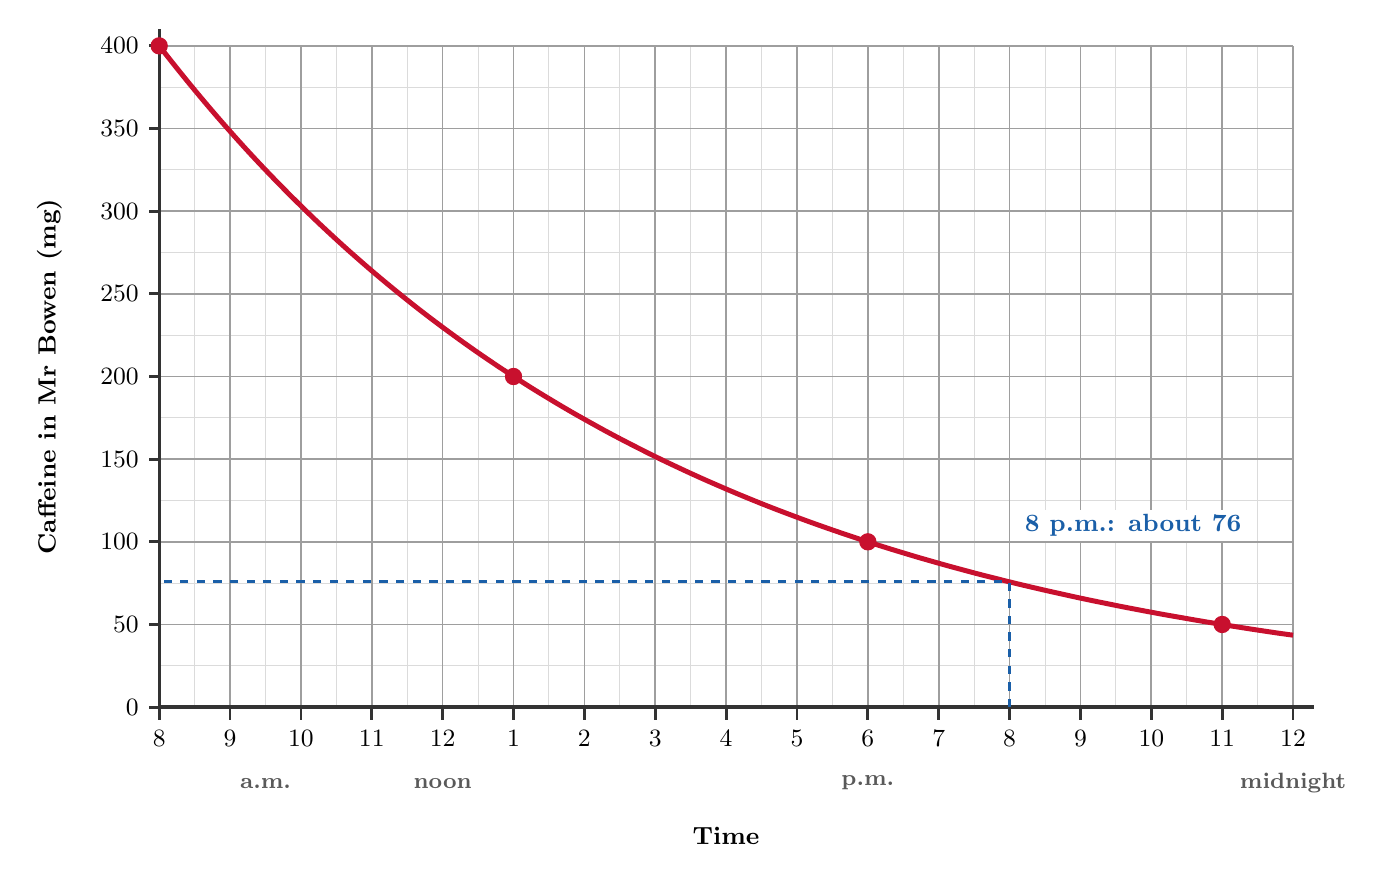
\begin{tikzpicture}[x=0.9cm, y=0.021cm]
  \bowenaxes
  \draw[cbred, line width=1.8pt] plot[domain=0:16, samples=80, smooth]
    (\x, {400*0.5^(\x/5)});
  \foreach \h/\v in {0/400, 5/200, 10/100, 15/50}
    \fill[cbred] (\h,\v) circle (0.11cm);
  \draw[cbblue, line width=1pt, dashed] (12,0) -- (12,75.8) -- (0,75.8);
  \node[right, font=\small\bfseries, text=cbblue, fill=white, inner sep=1.5pt]
    at (12.15,110) {8~p.m.: about 76};
\end{tikzpicture}
\end{center}

\noindent{\small Look for a \textbf{curve}. Straight lines between the dots
are the common one; they make A5(b) come out at 80 instead of 76.}

\qhead[cbred]{A5}{Read the graph}
\noindent (a) between \textbf{100} and \textbf{50} mg \sep (b) about
\textbf{76} mg (accept 70--85)

\smallskip
\noindent{\small (a) is deck slide 5's method, said in words: name the two
points either side before reading between them. 80 is fine from a student
who drew straight lines; ask them why the curve sits a little lower.}

\qhead[cbred]{A6}{The title question}
\noindent\textit{Mr Bowen is still awake because at 11~p.m. he still has
50 mg of caffeine in his body. That is half a cup of coffee.}

\smallskip
\noindent{\small Check for the number \emph{and} the comparison. ``Because he
drank coffee'' is true and is not the answer.}

\qhead[cbred]{B1--B4}{The interview and the halving table}
\noindent{\small No single answer. Mark in this order, and stop at the first
thing that is missing --- it is the thing to send back:}
\begin{enumerate}
  \item A real person, named by relationship (``my mother''), one drink with
    its size and time, and a bedtime.
  \item B2: an amount in mg and a ticked source. A blank is not acceptable;
    any honest number is.
  \item B3 starts at the drink's time, adds 5 hours a box, and halves each
    time. \textbf{Check the clock}: 9~a.m.\ $+$ 5 hours is 2~p.m., not
    ``14'' or ``14~p.m.''; 8~p.m.\ $+$ 5 hours is 1~a.m. The tea example
    crosses noon and midnight on purpose.
  \item B4: the two boxes either side of bedtime, their two numbers, and a
    number between them. If bedtime falls exactly on a box, that box is the
    answer.
\end{enumerate}

\noindent{\small \textbf{Numbers to sanity-check against} (all approximate;
the point is that the student found one and said where): Sting, 330 ml, about
50--85 mg (the Vietnamese label gives a range per litre, worth a minute in
class) \sep cola, 330 ml can, about 30--35 mg \sep Red Bull, 250 ml can, about
50--80 mg depending on the version \sep one espresso shot, about 60--75 mg
\sep Vietnamese iced coffee, about 100--200 mg (robusta, and very variable)
\sep a cup of black or green tea, about 30--50 mg.}

\qhead[cbred]{B5}{Compare with Mr Bowen}
\noindent{\small Needs a number, more or less, and \emph{because} with a
reason from their own table: a bigger drink, a smaller drink, or a drink
earlier or later in the day. Most adults who drink one morning coffee will be
well under 50 mg; an afternoon Sting will not. That sheet is worth showing
the class (without the name).}

\qhead[cbred]{B6}{Is your number right?}
\noindent{\small Any of the three, written as a sentence. ``I might have made
a mistake'' is not a limitation of the model --- ask which part of the model.
A student who adds a reason of their own (the caffeine takes time to get into
the blood; yesterday was not a normal day) deserves the credit.}

\qhead[cbred]{C1}{The halving chain}
\noindent 100\%, 50\%, \textbf{25\%, 12.5\%, 6.25\%} \sep 0, 5\,700,
\textbf{11\,400, 17\,100, 22\,800} years

\qhead[cbred]{C2}{The museum}
\renewcommand{\arraystretch}{1.2}
\noindent\begin{tabularx}{\linewidth}{@{}p{3.4cm}p{2.2cm}p{1.4cm}p{0.6cm}L@{}}
  bear bone & yes & 25\% & 2 & \textbf{11\,400} \\
  wooden spear & yes & 12.5\% & 3 & \textbf{17\,100} \\
  stone axe & \textbf{no} & --- & --- & \textbf{does not work} \\
  \textit{T.\ rex} tooth & \textbf{yes} & 0\% & --- & \textbf{does not work}
    (too old) \\
\end{tabularx}

\smallskip
\noindent{\small \textbf{The \textit{T.\ rex} is the question.} Expect ``no''
under \emph{Was it ever alive?} because it is dead now. It \emph{was} alive;
it is too old (deck slide 19: 66 million years, over 11\,000 half-lives). A
student who says ``it was alive, so it works'' has missed the 50\,000-year
limit.}

\qhead[cbred]{C3}{Why does it not work?}
\noindent (a) \textbf{alive} \sep (b) \textbf{old}

\qhead[cbred]{D1}{How old is the Sun?}
\noindent (a) \textbf{hydrogen} into \textbf{helium} \sep (b) \textbf{35.5}\%
\sep (c) \textbf{yes} \sep (d) about \textbf{4.6}; about \textbf{4.6}

\smallskip
\noindent{\small (c): 34 is close to 35.5, so about half is gone --- deck
slide 21's hydrogen bar. Do not let ``half-life of 4.6 billion years'' creep
in: the Sun burns its hydrogen as fuel; it does not decay. The deck says
``about half gone in 4.6 billion years'', and so does this sheet. (b) is
there because ``half of 71'' is a real step; 35 or 36 is fine.}

\qhead[cbred]{D2}{Three clocks}
\noindent Caffeine $\to$ \textbf{every 5 hours} \sep Carbon-14 $\to$
\textbf{every 5\,700 years} \sep the Sun $\to$ \textbf{4.6 billion years}
\sep order: \textbf{caffeine, carbon-14, the Sun}

\qhead[cbred]{E1}{Plan your letter}
\noindent (a) \textbf{50} mg; \textbf{adenosine} \sep (b) \textbf{3~p.m.}
\sep (c) \textbf{100, 50, 25} mg

\smallskip
\noindent{\small (b) is 11~p.m.\ minus 8 hours; expect 4~p.m.\ or 2~p.m.\
from a student counting on their fingers. (c) is the advice with a number in
it: one cold brew instead of two halves his bedtime caffeine, 50 mg to
25 mg. A student who writes 100 at 11~p.m.\ halved once for the whole day.}

\smallskip
\noindent{\small \textbf{Expect: ``50 mg is less than 100 mg, so he should
sleep.''} Good thinking, and worth a minute in class. The 100 mg is a cup
drunk \emph{near} bedtime, and it is ``can'', not ``will'': some adults are
kept awake by less. His real problem is the size of the drink: 400 mg is four
cups, so 15 hours was not enough --- the guide's ``a bigger drink needs
longer''.}

\qhead[cbred]{E2}{A letter to Mr Bowen}
\noindent{\small No sentence starter on purpose: the students begin it
themselves. Mark the six ticks in order; the first one missing is the thing
to send back. The advice must come with a \emph{why}. A model answer:}

\smallskip
\noindent\textit{Dear Mr Bowen, You drank 400 mg of caffeine at 8 a.m.
That is four cups of coffee. Caffeine has a half-life of 5 hours, so at
11 p.m. you still have 50 mg in your body. Caffeine blocks adenosine, so your
brain does not feel sleepy. Please drink only one cold brew, because then you
will have 25 mg at bedtime, not 50 mg. From, \ldots}

\smallskip
\noindent{\small \textbf{The guide's facts, and where they come from.}
(1--2) Adenosine builds up while we are awake and makes us sleepy; caffeine
blocks its receptors. (3) Caffeine delays sleep and adds waking in the
night. (4) European Food Safety Authority, \textit{Scientific Opinion on the
safety of caffeine} (2015): single doses of 100 mg (1.4 mg per kg for a 70 kg
adult) may delay sleep and shorten it in some adults, especially close to
bedtime. The 50 mg for a child is our arithmetic, not an EFSA figure: the
same 1.4 mg per kg for a 35--40 kg Year 7. For the whole day, Health Canada's
maximum for ages 10--12 is 85 mg. (5) Gardiner et al., \textit{Sleep Medicine
Reviews} 2023, a meta-analysis: a cup of coffee (about 107 mg) at least
8.8 hours before bed to avoid losing sleep, and a 217 mg dose at least
13.2 hours. Drake et al.\ (2013) found 400 mg even 6 hours before bed cut
sleep by more than an hour, which is why the sheet says 8, not the 6 often
quoted. (6) US National Sleep Foundation: 9--11 hours for ages 6--13 (the
American Academy of Sleep Medicine says 9--12 to age 12, 8--10 from 13).}

\fi

\end{document}
